\documentclass[tikz,border=3pt]{standalone}
% Shared preamble for the v2 figures.
% Fonts: acmart's pdfLaTeX set (Libertine text, newtxmath[libertine]) when
% installed; otherwise Latin Modern. Recompile once Libertine is installed.
\usepackage[T1]{fontenc}
\usepackage{amsmath}
\IfFileExists{libertine.sty}{%
  \IfFileExists{newtxmath.sty}{%
    \usepackage[tt=false,type1=true]{libertine}%
    \usepackage[libertine]{newtxmath}%
  }{\usepackage{lmodern}}%
}{\usepackage{lmodern}}
% Colours: Okabe--Ito-derived, distinguishable in greyscale by luminance
% and always paired with a second cue (line weight, dash, marker shape).
\definecolor{editblue}{HTML}{193E57}  % dark: paths, peeling steps, branch
\definecolor{lawgray}{HTML}{81888C}   % mid grey: constraint sets, context
\definecolor{pointver}{HTML}{D55E00}  % vermillion: forced points, blocks
\newcommand{\lab}[1]{\mathsf{#1}}     % labels in sans serif

\usetikzlibrary{arrows.meta,positioning,calc}


\newcommand{\wt}{\mathrm{wt}}
\begin{document}
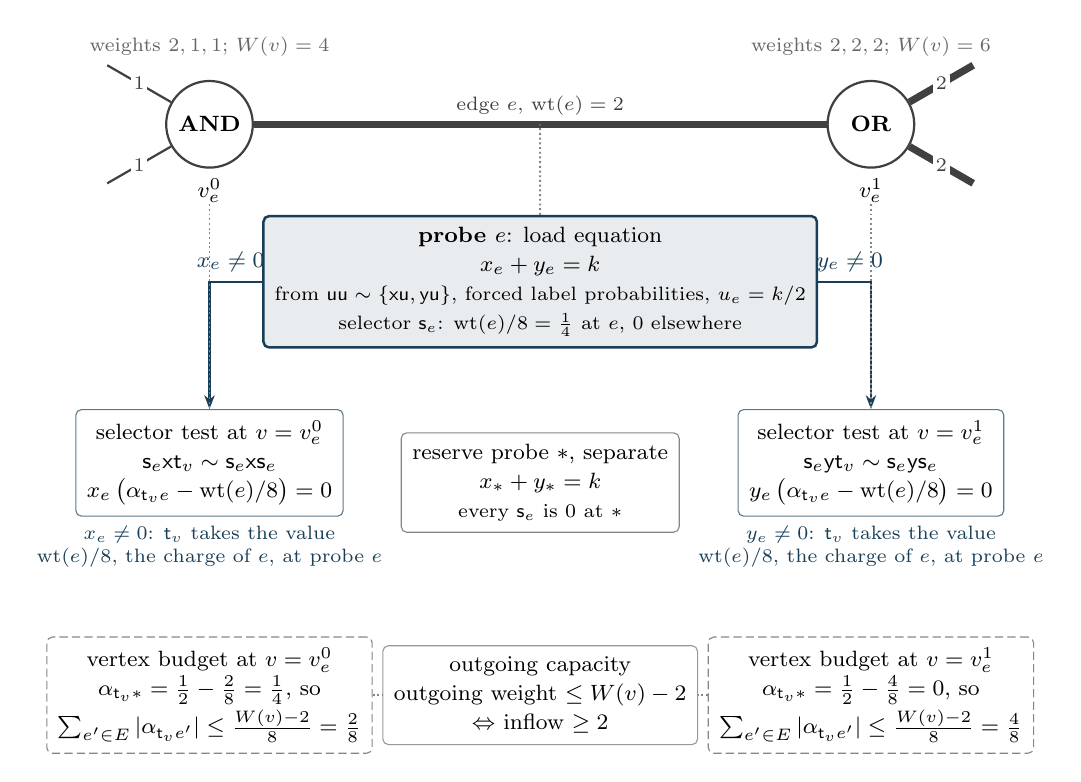
\begin{tikzpicture}[
  every node/.style={font=\small},
  vtx/.style={draw=black!75, circle, line width=0.8pt, minimum size=11mm,
    inner sep=0pt, font=\footnotesize\bfseries, fill=white},
  w2/.style={black!75, line width=2.6pt},
  w1/.style={black!75, line width=0.8pt},
  box/.style={draw=editblue!70, rounded corners=2pt, inner sep=4pt,
    align=center, fill=white, font=\footnotesize},
  probebox/.style={box, fill=editblue!10, draw=editblue, line width=0.9pt},
  budget/.style={box, draw=lawgray, dash pattern=on 3pt off 1.5pt},
  link/.style={editblue, line width=0.9pt, -{Stealth[length=5pt]}},
  ref/.style={lawgray, line width=0.7pt, densely dotted},
  wlab/.style={font=\scriptsize, fill=white, inner sep=1pt},
]
%---------------------------------------------------------------- NCL fragment
\node[vtx] (and) at (2.2,6.3) {AND};
\node[vtx] (or)  at (10.6,6.3) {OR};
\node[font=\footnotesize, anchor=north] at (and.south) {$v_e^0$};
\node[font=\footnotesize, anchor=north] at (or.south)  {$v_e^1$};
\draw[w2] (and) -- node[wlab, above=1pt] {edge $e$,\ $\wt(e)=2$} (or);
\draw[w1] (and) -- node[wlab] {1} ++(150:1.5);
\draw[w1] (and) -- node[wlab] {1} ++(210:1.5);
\draw[w2] (or)  -- node[wlab] {2} ++(30:1.5);
\draw[w2] (or)  -- node[wlab] {2} ++(-30:1.5);
\node[font=\scriptsize, text=black!60, anchor=south] at ([yshift=5pt]and.north)
  {weights $2,1,1$;\ $W(v)=4$};
\node[font=\scriptsize, text=black!60, anchor=south] at ([yshift=5pt]or.north)
  {weights $2,2,2$;\ $W(v)=6$};

%---------------------------------------------------------------- the probe e
\node[probebox] (probe) at (6.4,4.3)
  {\textbf{probe $e$}: load equation\\[1pt]
   $x_e+y_e=k$\\[1pt]
   {\scriptsize from $\lab{u}\lab{u}\sim\{\lab{x}\lab{u},\lab{y}\lab{u}\}$, forced label probabilities, $u_e=k/2$}\\[1pt]
   {\scriptsize selector $\lab{s}_e$: $\wt(e)/8=\frac14$ at $e$, $0$ elsewhere}};
\draw[ref] (probe.north) -- ($(and)!0.5!(or)$);

%---------------------------------------------------------------- selector tests
\node[box] (selA) at (2.2,2.0)
  {selector test at $v=v_e^0$\\[1pt]
   $\lab{s}_e\lab{x}\lab{t}_v\sim\lab{s}_e\lab{x}\lab{s}_e$\\[1pt]
   $x_e\,\bigl(\alpha_{\lab{t}_v e}-\wt(e)/8\bigr)=0$};
\node[box] (selB) at (10.6,2.0)
  {selector test at $v=v_e^1$\\[1pt]
   $\lab{s}_e\lab{y}\lab{t}_v\sim\lab{s}_e\lab{y}\lab{s}_e$\\[1pt]
   $y_e\,\bigl(\alpha_{\lab{t}_v e}-\wt(e)/8\bigr)=0$};
\draw[link] (probe.west) -| node[pos=0.3, above, font=\footnotesize] {$x_e\neq0$} (selA.north);
\draw[link] (probe.east) -| node[pos=0.3, above, font=\footnotesize] {$y_e\neq0$} (selB.north);
\draw[ref] (and.south) ++(0,-0.45) -- (selA.north);
\draw[ref] (or.south)  ++(0,-0.45) -- (selB.north);
\node[font=\scriptsize, text=editblue, align=center, anchor=north] at (selA.south)
  {$x_e\neq0$: $\lab{t}_v$ takes the value\\$\wt(e)/8$, the charge of $e$, at probe $e$};
\node[font=\scriptsize, text=editblue, align=center, anchor=north] at (selB.south)
  {$y_e\neq0$: $\lab{t}_v$ takes the value\\$\wt(e)/8$, the charge of $e$, at probe $e$};

%---------------------------------------------------------------- vertex budgets
\node[budget] (budA) at (2.2,-0.95)
  {vertex budget at $v=v_e^0$\\[1pt]
   $\alpha_{\lab{t}_v\ast}=\frac12-\frac28=\frac14$, so\\[1pt]
   $\sum_{e'\in E}|\alpha_{\lab{t}_v e'}|\le\frac{W(v)-2}{8}=\frac28$};
\node[budget] (budB) at (10.6,-0.95)
  {vertex budget at $v=v_e^1$\\[1pt]
   $\alpha_{\lab{t}_v\ast}=\frac12-\frac48=0$, so\\[1pt]
   $\sum_{e'\in E}|\alpha_{\lab{t}_v e'}|\le\frac{W(v)-2}{8}=\frac48$};

\node[box, draw=black!40, align=center] (cap) at (6.4,-0.95)
  {outgoing capacity\\[1pt]
   outgoing weight $\le W(v)-2$\\[1pt]
   $\Leftrightarrow$ inflow $\ge2$};
\draw[ref] (budA.east) -- (cap.west);
\draw[ref] (budB.west) -- (cap.east);

%---------------------------------------------------------------- reserve probe
\node[box, draw=lawgray, align=center] (res) at (6.4,1.75)
  {reserve probe $\ast$, separate\\[1pt]
   $x_\ast+y_\ast=k$\\[1pt]
   {\scriptsize every $\lab{s}_e$ is $0$ at $\ast$}};
\end{tikzpicture}
\end{document}
